\chapter{Modeling of Train Operations}
\label{chap:ModelingOfTrainOperations}
\par\noindent
\textit{\textbf{Introduction}} Chapter \ref{chap:FundamentalsOfRailwayVehicleEngineering} has established the theoretical model of the train braking process. It will serve as a foundation to build a practical model suitable for conducting actual simulations. 

\section{Matlab Simulink}
\label{sec:MatlabSimulink}
The model has been built utilizing the software Matlab Simulink by Mathworks. It offers several distinct advantages: It uses a graphical block diagramming tool which makes it very intuitive to use. At the same time, various official and third-party add-on libraries make it very versatile. Most importantly, as it is tightly integrated with the Matlab environment, it can be used for both modeling and simulating dynamical systems, like the braking process of a train.

\section{Initial Model}
\label{sec:InitialModel}
\par\noindent
Looking back at chapter \ref{chap:FundamentalsOfRailwayVehicleEngineering}, the aim is to build a model for the braking process of a freight train. An initial model of a single braking procedure, kindly provided by Dr. Raphael Pfaff, will serve as a basis. Most of the components previously designed in chapter \ref{chap:FundamentalsOfRailwayVehicleEngineering} can already be found therein.  

\begin{figure}[H]
	\centering
	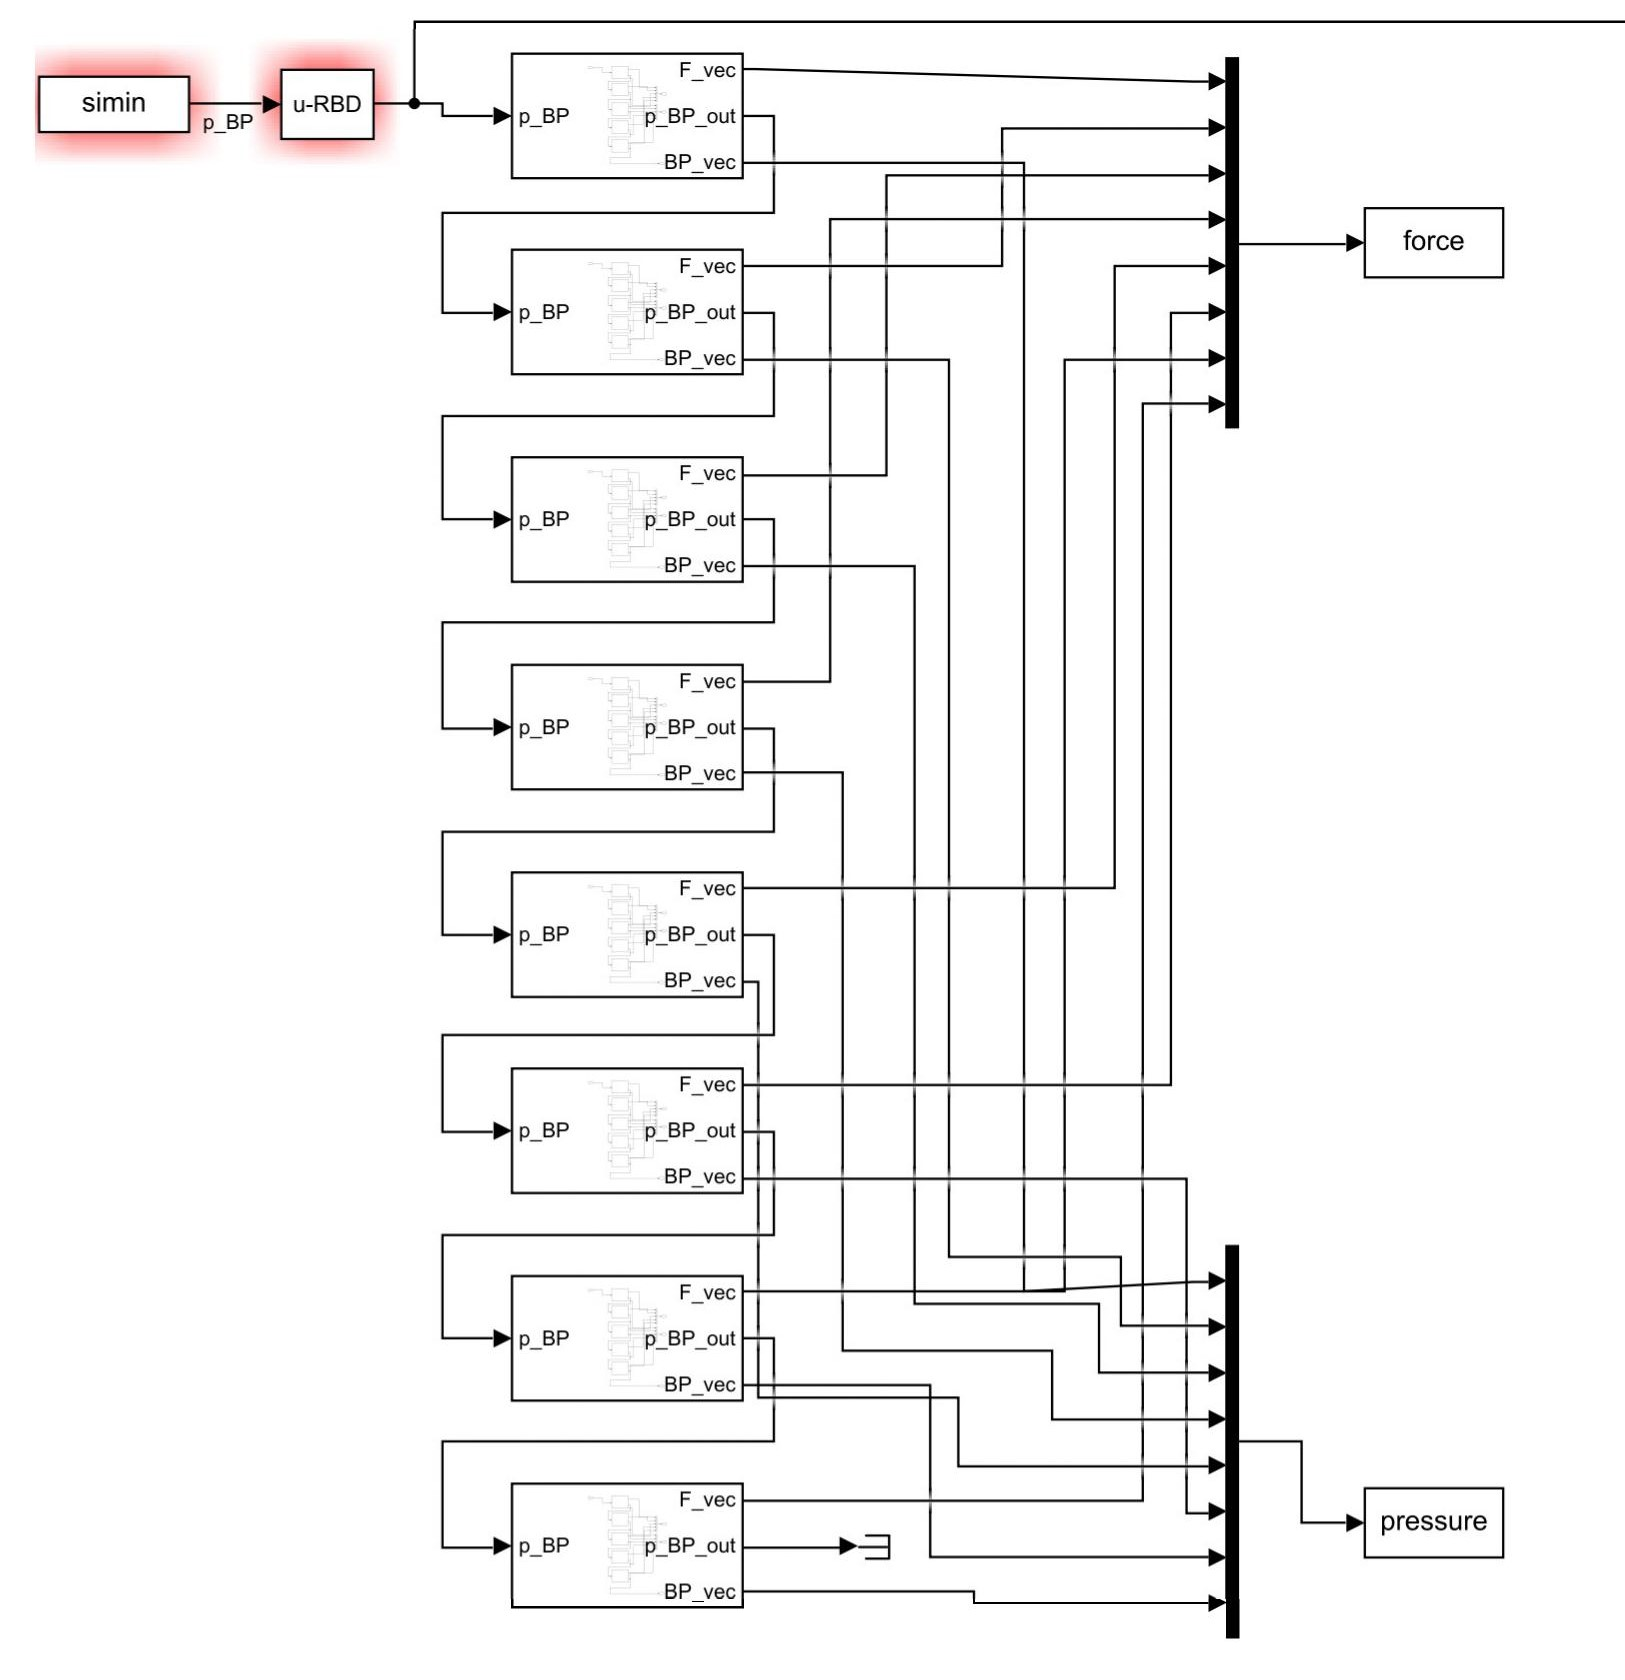
\includegraphics[width=\linewidth]{./pic/initmodel_whole}
	\caption{Initial Model}
	\label{fig:initmodel_whole}
\end{figure}

\par\noindent
Figure \ref{fig:initmodel_whole} shows a model of a freight train of fixed length, consisting of 40 wagons in total. For better readability, five wagons are condensed into one subsystem each, marked by the red rectangle. The subsystems are interconnected by a brake pipe, marked by the green arrow. They have one input port for the incoming pressure on the brake pipe, and three output ports, one for the pipe connection to the next subsystem, and two for recording brake pressure and brake force (marked by the pink and blue arrows, respectively). A depiction of a subsystem can be found in appendix \ref{fig:initmodel_subsys}.  

\begin{figure}[H]
	\centering
	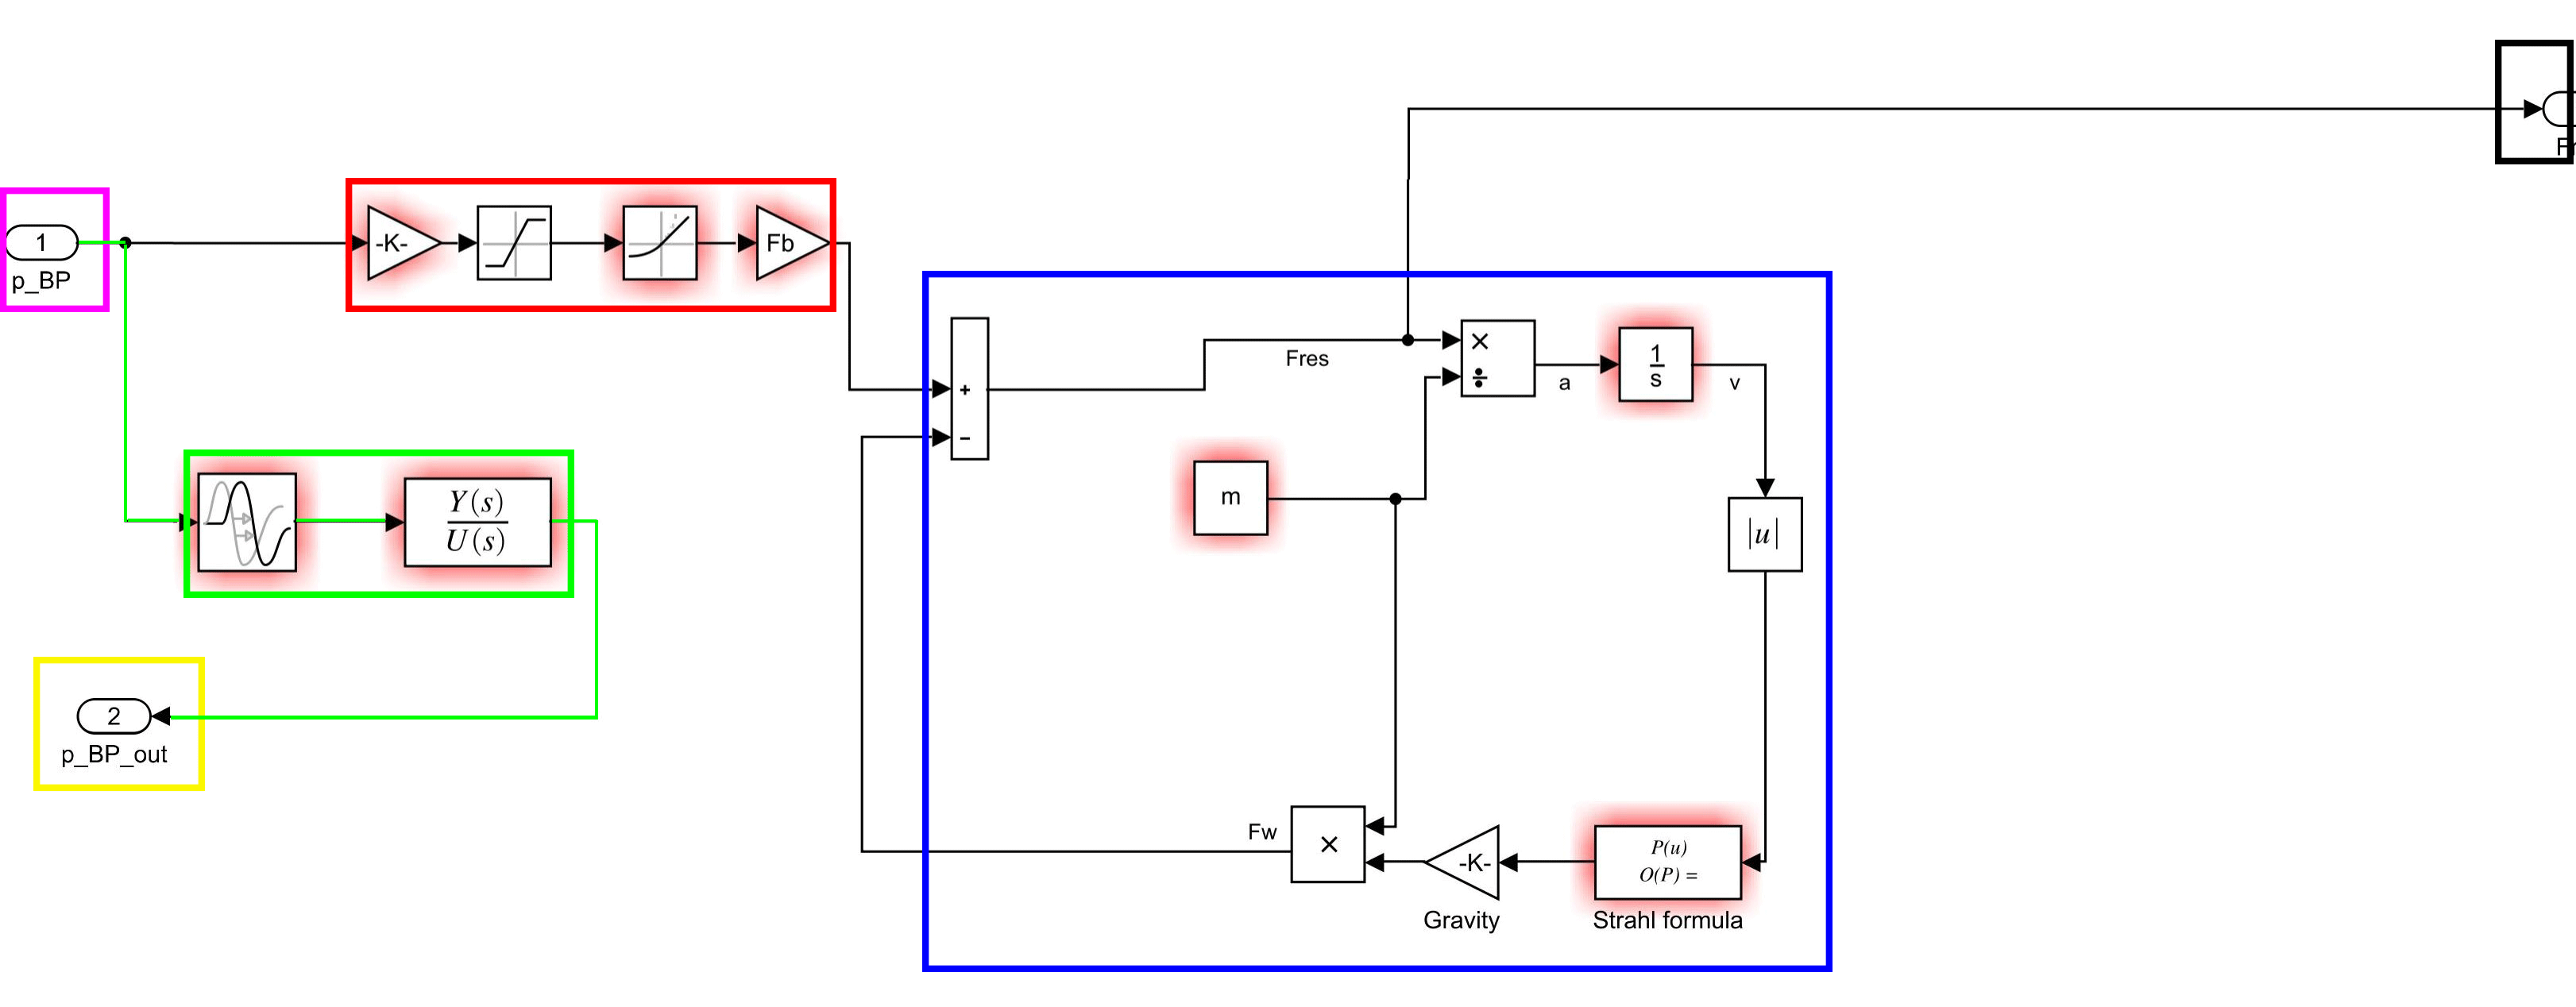
\includegraphics[width=\linewidth]{./pic/initmodel_wagon}
	\caption{Initial Model - Wagon}
	\label{fig:initmodel_wagon}
\end{figure}

\par\noindent
Figure \ref{fig:initmodel_wagon} shows a model of a freight wagon. It already encompasses several of the model variables defined in section \ref{sec:InherentFactors}. The brake pipe ${\mathcal{M}}_{bp}$ is represented by the green arrows. It leads from input port (pink rectangle) to output port (yellow rectangle); the propagation delay is realized by a transport delay block (green rectangle), using propagation velocity $v_{bp}$ and wagon length $l_{bp}$. The brake pressure $p_{bp}$ is the value of the signal traveling through the connection. Note that in the simulation, the signal value for $p_{bp}$ is the difference between regular operating pressure and actual pressure, e.g. if simulated pressure on the brake pipe is 3.5 bar, the signal value is $3.5 - 5 = -1.5$.
\par
The brake cylinder ${\mathcal{M}}_{bc}$ is represented by the red rectangle. The pressure on the brake pipe $p_{bp}$ is converted into a coefficient between zero and one, where zero equals no brakes applied, or $p_{bp} = 5$, and one equals full braking pressure, or $p_{bp} = 3.5$. The exact formula is this:

\begin{align*}
p_{bc} = p_{bp} \cdot \frac{-1}{5-3.5}
\end{align*}

\noindent
So for a braking pressure of 4 bar, the coefficient would be $(4 - 5) \cdot \frac{-1}{5-3.5} = -1 \cdot \frac{-1}{1.5} = \frac{2}{3}$. A rate limiter block accounts for the brake cylinder's filling time $t_{bc}$. Finally, the braking force is calculated by multiplying the maximum braking force, which is mainly dependent on the wagon mass $m$ [train braking, 22]. So for the braking pressure, we have:

\begin{align*}
F_{b} = F_{b,max} \cdot p_{bc}
\end{align*}

\noindent
The final component is the factoring in of the driving resistance of the train, utilizing Strahl's formula. This is represented by the blue rectangle. By continuous-time integration of the acceleration, which is calculated according to Newton's second law of motion ($a = \frac{F}{m})$, it is possible to determine the velocity, which in turn allows for the calculation of the force generated by the driving resistance, This force is then added to the braking force and fed into an output port, marked with the black rectangle.
\par
Regarding simulation, this initial model is only fit for one single braking process, where a train of fixed length and fixed composition, brakes from an initial velocity all the way to a halt; the only variation is the pressure on the brake pipe, which is also the sole input for the simulation. Appendix \ref{fig:initmodel_input} shows how that input might look like.

\section{Model Expansion}
\label{sec:ModelExpansion}

\par\noindent
This initial model is however not of sufficient detail. Where it merely simulates a single, rather undynamic braking process, the goal is the simulation of a train ride, with alternating phases of braking and accelerating. The model should furthermore factor in more components of the theoretical model ${\mathcal{M}}$ discussed in chapter \ref{chap:FundamentalsOfRailwayVehicleEngineering}, as well as allow for the recording of more properties specific to the braking process. For that purpose, the model has to be expanded. The simulation input needs to be changed in order to allow for the simulation of a train ride. Previously, it being only one braking process, using braking pressure as input was the obvious choice. This will be replaced by a track profile, according to which the train either engages its brakes, or accelerates. This will be discussed in further detail in chapter \ref{chap:DataGeneration}.
\par
In the initial model, the train is only able to decelerate by engaging its brakes. To allow for acceleration, it is necessary to expand the model accordingly. This may be realized by a rather simple two-point controller, which means the train is either accelerating or decelerating. The decision on whether to engage brakes or apply traction force at a particular point in time is made utilizing the track profile: If the current velocity of the train $v_{real}$ is greater than the maximum allowed velocity $v_{max}$ at that time, the train engages its brakes by lowering the pressure on the brake pipe $p_{bp}$. If $v_{real}$ is less than $v_{max}$, the train applies a traction force $F_{t}$ in order to increase speed. Both $p_{bp}$ and $F_{t}$ scale with the discrepancy between $v_{real}$ and $v_{max}$. This means the higher the value of $v_{dif}$ is, the more pressure is vented from the brake pipe (or the more traction force is applied). This prevents the train from overcompensating, for example applying full braking pressure to decrease velocity by $2 \; \frac{m}{s}$. Notice there is actually no case for when $v_{real}$ equals $v_{max}$, i.e. $v_{dif} = 0$. One might expect that this would lead to the train constantly oscillating between accelerating and decelerating, but in practice this does not occur, and it is thus unnecessary to account for that case.

\begin{figure}[H]
	\centering
	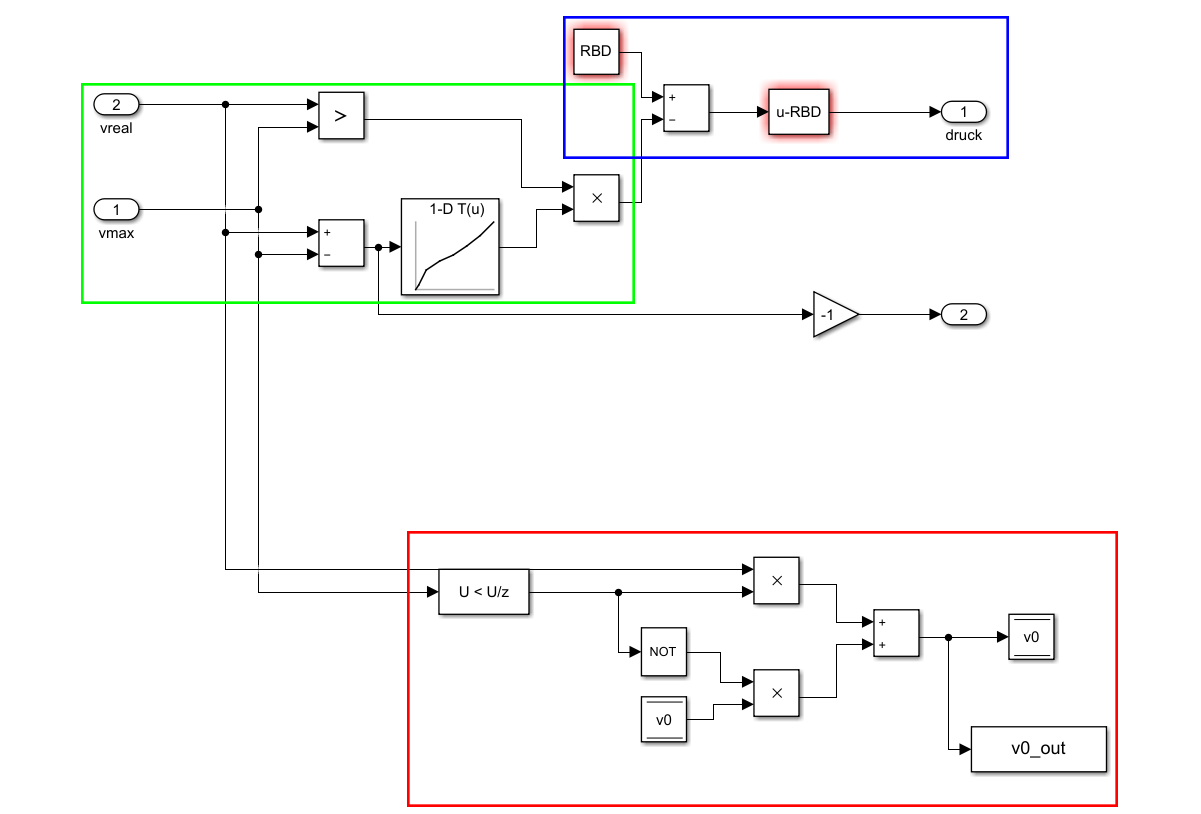
\includegraphics[width=\linewidth]{./pic/expandedmodel_pressure}
	\caption{Expanded Model - Pressure Calculation}
	\label{fig:expandedmodel_pressure}
\end{figure}

\par\noindent
Figure \ref{fig:expandedmodel_pressure} shows the subsystem responsible for the calculation of the braking pressure $p_{bp}$. The difference between $v_{real}$ and $v_{max}$ is used as input for a one-dimensional lookup table, which in essence is a step-function mapping different input values to discrete output values. 

\begin{equation}
\label{eq:lookuptable}
H(n) =
\begin{cases}
0.1 & \text{if $n=1$} \\
0.7 & \text{if $n=15$} \\
0.8 & \text{if $n=20$} \\
\text{..}
\end{cases}
\end{equation}

\noindent
Equation \ref{eq:lookuptable} is an example for how this function might look like. The input parameter $n$ stands for the discrepancy between actual and maximum velocity $v_{dif}$, and the output of the $H(n)$ represents the amount of pressure to vent from the brake pipe. This allows for adjusted braking, where $p_{bp}$ is directly proportional to $v_{dif}$.
\par
To account for the train only engaging its brakes in case its current velocity is higher than the maximum allowed velocity, a relational operator $>$ is used to compare $v_{real}$ to $v_{max}$.

\begin{equation}
\label{eq:brakingpressure}
P(n,t) = H(n) \cdot (v_{real}(t) > v_{max}(t))
\end{equation}

\noindent
Equation \ref{eq:brakingpressure} describes the logic. The braking pressure for a velocity discrepancy $n$ at a point in time $t$ equals the result of $H(n)$ (equation \ref{eq:lookuptable}) multiplied with the result of the relational operation comparing $v_{real}(t)$ to $v_{max}(t)$, which is 1 if $v_{real}(t)$ is greater than $v_{max}(t)$, and otherwise 0. This ensures that $P(n,t)$ is zero when the train's velocity is lower than the maximum allowed velocity, and thus no pressure is vented from the brake pipe, and no brakes are engaged. This part of the system is marked by the green rectangle in figure \ref{fig:expandedmodel_pressure}. The blue rectangle marks the conversion of the braking pressure into a signal fit for further calculations, analogous to the initial model, discussed previously. Finally, the red rectangle marks the component for storing the initial velocity of a braking process, which is needed to calculate the braking distance further down the line. This is achieved by using a block to detect a decrease of $v_{max}$, i.e. the block outputs a signal of 1 or 0, accordingly. 

\begin{equation}
\label{eq:initialvelocity}
v_{0} = v_{real} \cdot b + v_{0,old} \cdot \bar{b}
\end{equation}

\noindent
Equation \ref{eq:initialvelocity} describes the logic. The initial velocity of a braking process $v_{0}$ equals the train's velocity multiplied with the result of the decrease detection block, denoted as $b$, added with the previously stored initial velocity $v_{0,old}$ multiplied with the inverse of $b$, denoted as $\bar{b}$. If there is a decrease of $v_{max}$, i.e. the train starts braking, we get $v_{0} = v_{real} \cdot 1 + v_{0,old} \cdot 0 = v_{real}$. In any other case, we get $v_{0} = v_{real} \cdot 0 + v_{0,old} \cdot 1 = v_{0,old}$, i.e. the value of $v_{0}$ does not change as no new braking process has begun.
\par
This completes the description of this subsystem. It is worthy to note that, reaching back to chapter \ref{chap:FundamentalsOfRailwayVehicleEngineering}, this is the practical implementation of the brake valve ${\mathcal{M}}_{bv}$.

\begin{figure}[H]
	\centering
	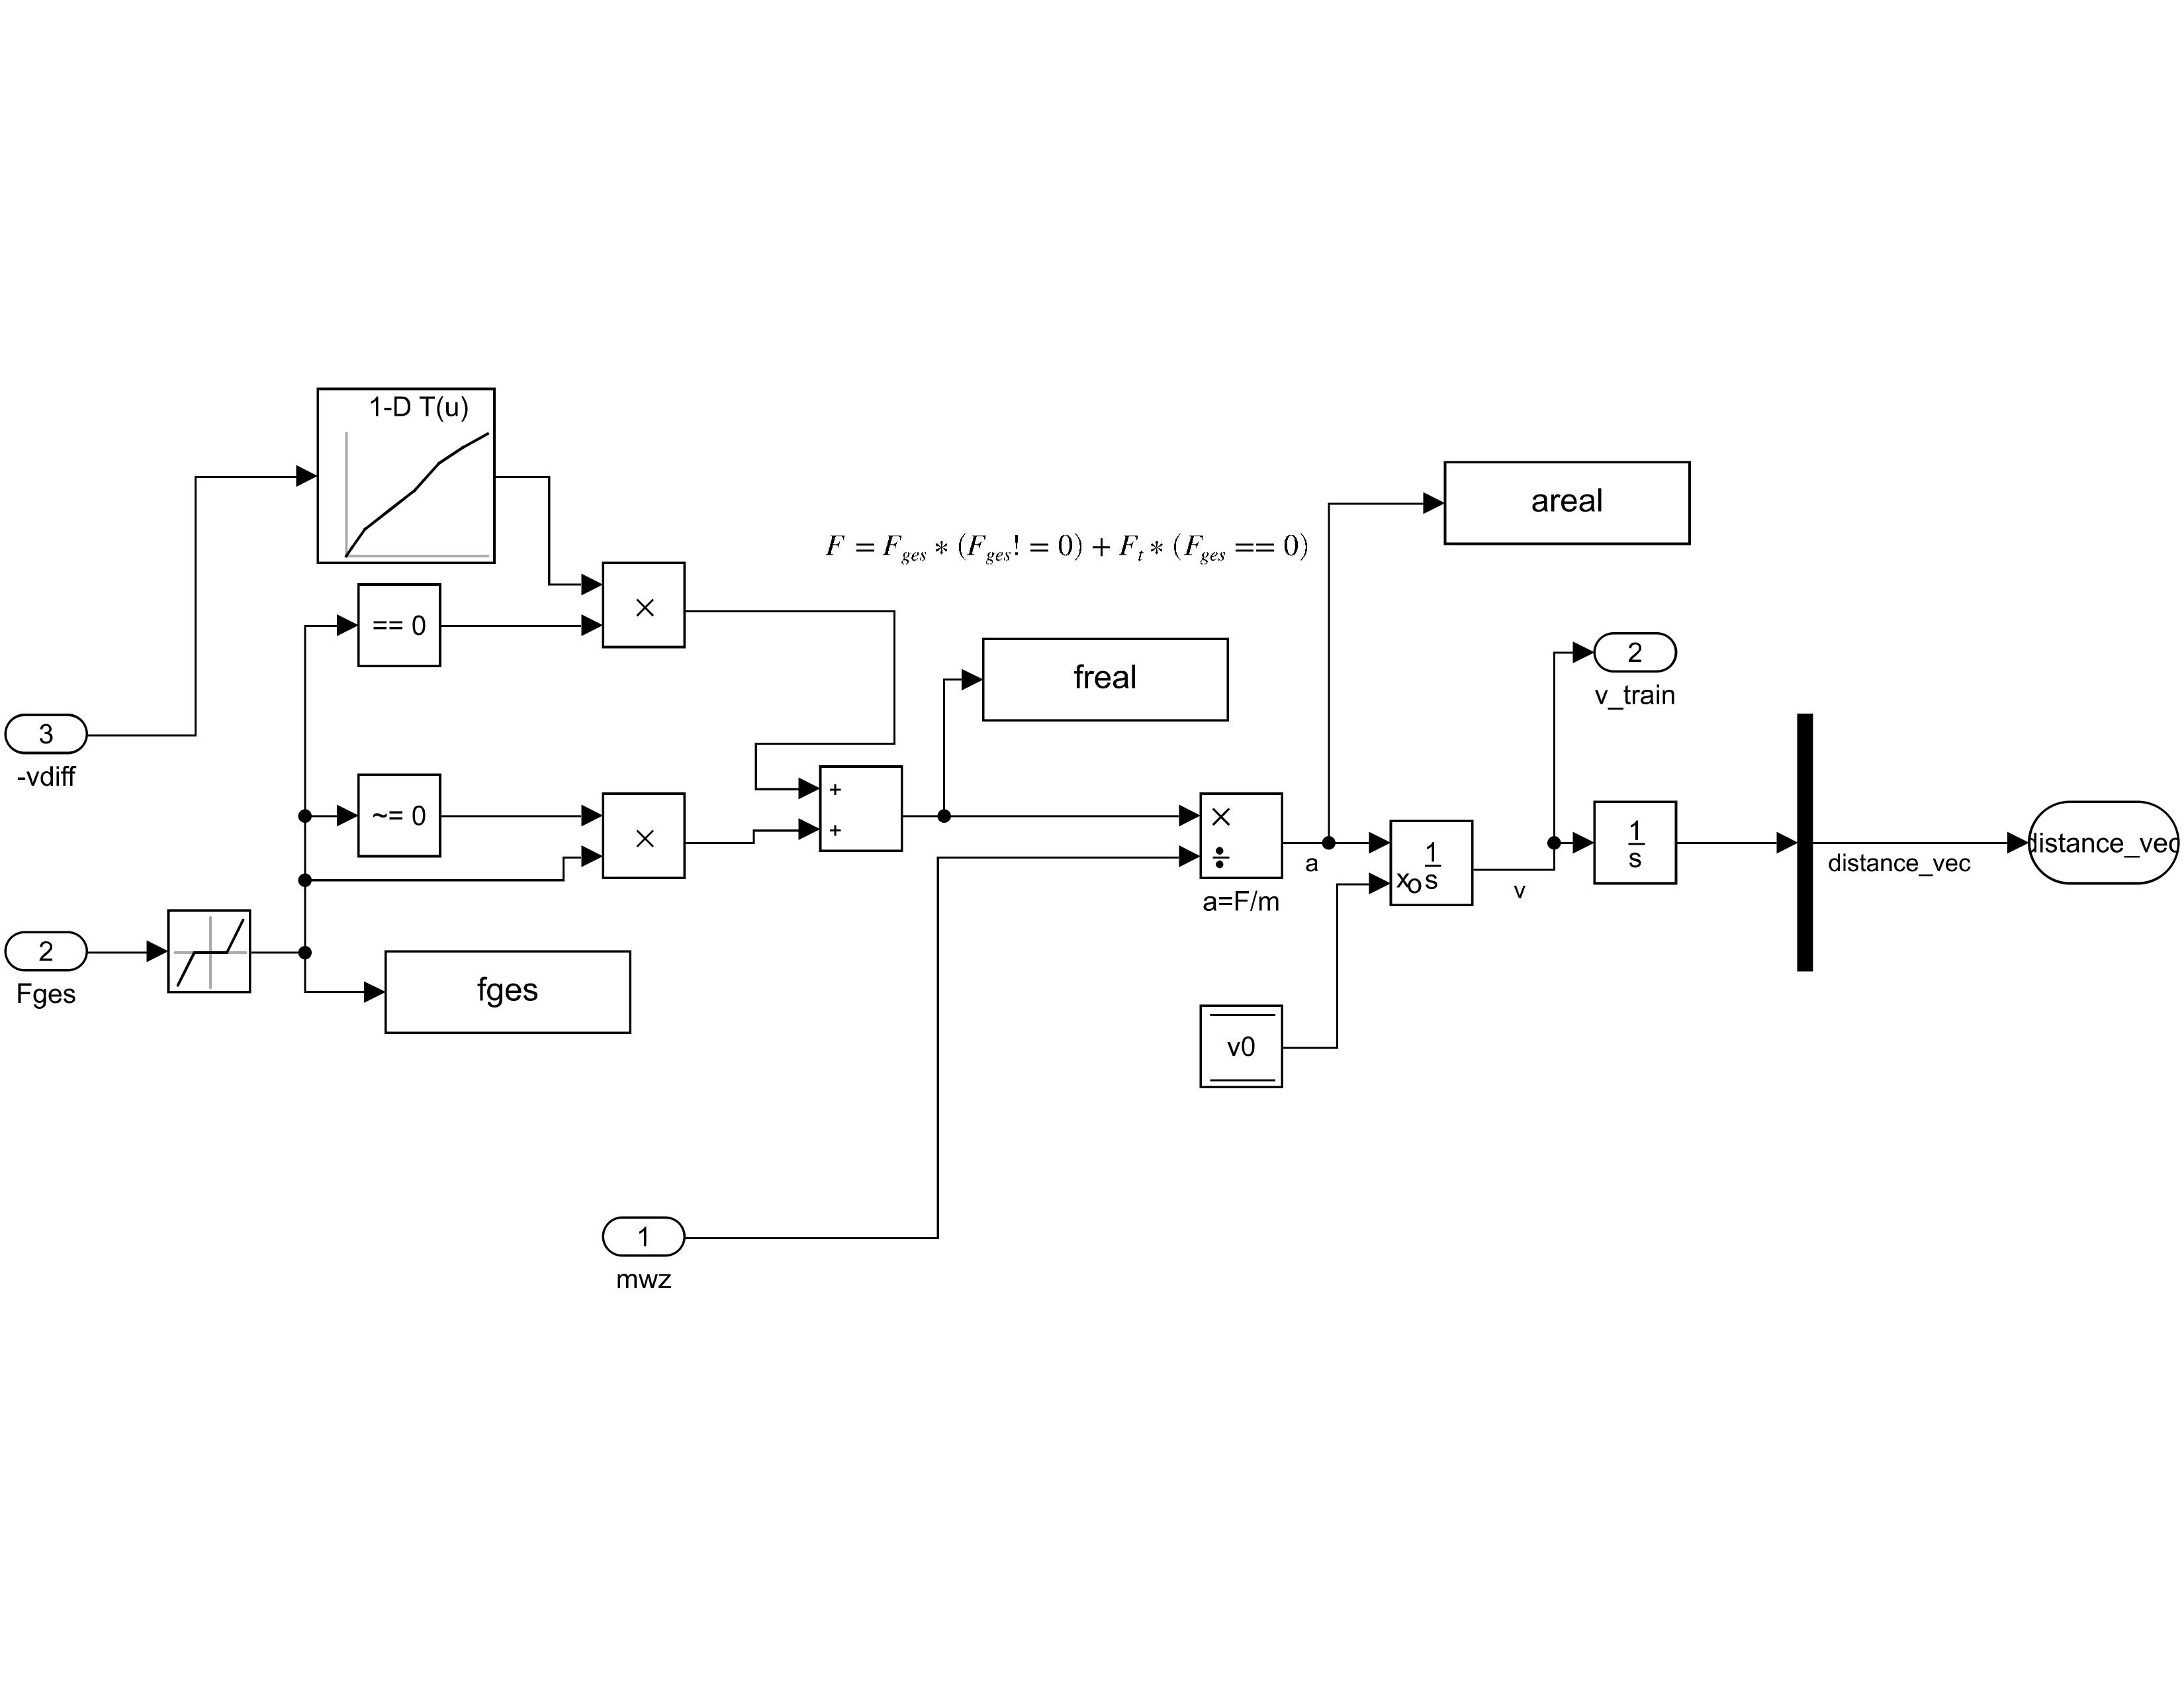
\includegraphics[width=\linewidth]{./pic/expandedmodel_force}
	\caption{Expanded Model - Traction Force Calculation}
	\label{fig:expandedmodel_force}
\end{figure}

\par\noindent
Figure \ref{fig:expandedmodel_force} shows the subsystem responsible for the calculation of the traction force, the train's acceleration, the train's velocity and the train's traveled distance. The applied traction force scales with $v_{dif}$ in a similar fashion to how $p_{bp}$ does. Again, a one-dimensional lookup table is used to calculate the appropriate value for $F_{t}$.

\begin{equation}
\label{eq:lookuptable2}
H(n) =
\begin{cases}
0.05 & \text{if $n=1$} \\
0.45 & \text{if $n=15$} \\
0.6 & \text{if $n=20$} \\
\text{..}
\end{cases}
\end{equation}

\noindent
Equation \ref{eq:lookuptable2} shows an example for how the function for the table might look like. The key difference to the calculation of the braking pressure is that the output values of the function are coefficients which are then multiplied with the maximum possible traction force, rather than raw values like in equation \ref{eq:lookuptable}. This part of the system is marked by the red rectangle. 
\par
Remember that we have established the train is at any given time either accelerating or decelerating. Since there is, as previously discussed, already a system in place to determine whether the train should engage its brakes, it now suffices to make the following examination: If the train is generating a braking force, i.e. $F_{b}$ is greater than zero, it will apply no traction force, and vice versa.
 
\begin{equation}
\label{eq:tracforce}
F_{t}(n,t) = (H(n) \cdot F_{t,max}) \cdot (F_{b}(n,t) == 0) 
\end{equation}

\noindent
Equation \ref{eq:tracforce} describes the logic. $F_{b}(t) == 0$ is a relational operation, the result being either 1 if there is a braking force at a particular point in time $t$, otherwise 0. We can apply the same logic to the braking force $F_{b}$:

\begin{equation}
\label{eq:brakeforce}
F_{b}(n,t) = F_{B}(n,t) \cdot (F_{b}(n,t) \neq 0)
\end{equation}

\noindent
With equations \ref{eq:tracforce} and \ref{eq:brakeforce} we can now determine the actual force applied at any given point in time $t$:

\begin{equation}
\label{eq:force}
F(n,t) = F_{t}(n,t) + F_{b}(n,t) 
\end{equation} 

\noindent
Since either of the summands is always zero, equation \ref{eq:force} outputs either the traction force or the braking force being applied at a point in time $t$, for a value of $v_{dif} = n$. This part of the system is marked by the blue rectangle, and together with the brake valve completes the system responsible for controlling the train.
\par\noindent
Let's reach back to our model ${\mathcal{M}}$ from chapter \ref{chap:FundamentalsOfRailwayVehicleEngineering}, in particular to three elements of its set of model variables $\{{\mathcal{V}}\}$: The train's acceleration $a$, its velocity $v$, and its braking distance $d$. Since we can now determine the applied force $F(n,t)$, it is now also possible to calculate the values of these three variables.

\begin{equation}
\label{eq:newton}
F = m \cdot a
\end{equation}

\noindent
Once again making use of Newton's second law of motion, we may calculate the value of $a$ by substituting $F(n,t)$ for $F$, and the combined mass of all wagons $m_{total}$ for $m$:

\begin{equation}
\label{eq:acceleration}
a = \frac{F(n,t)}{m_{total}}
\end{equation}
	
\noindent
The train's velocity may now be calculated by integration of its acceleration $a$. In simulink, this is achieved by feeding the signal value of $a$ into a continuous-time integration block:

\begin{equation}
\label{eq:velocity}
v = \int a \; da
\end{equation}

\noindent
Finally, the train's braking distance can be calculated by integration of its velocity $v$. This is once again achieved by usage of a continuous-time integration block:

\begin{equation}
\label{eq:distance}
d = \int v \; dv
\end{equation}

\noindent
This part of the system is marked by the green rectangle. This also completes the description of this subsystem. Looking back at our model ${\mathcal{M}}$, the last elements of $\{{\mathcal{V}}\}$ left to deal with are the brake pipe ${\mathcal{M}}_{bp}$, the brake cylinder ${\mathcal{M}}_{bc}$, the wagon mass $m$, the train composition $comp$, and finally the braking force $F_{b}$.

\begin{figure}[H]
	\centering
	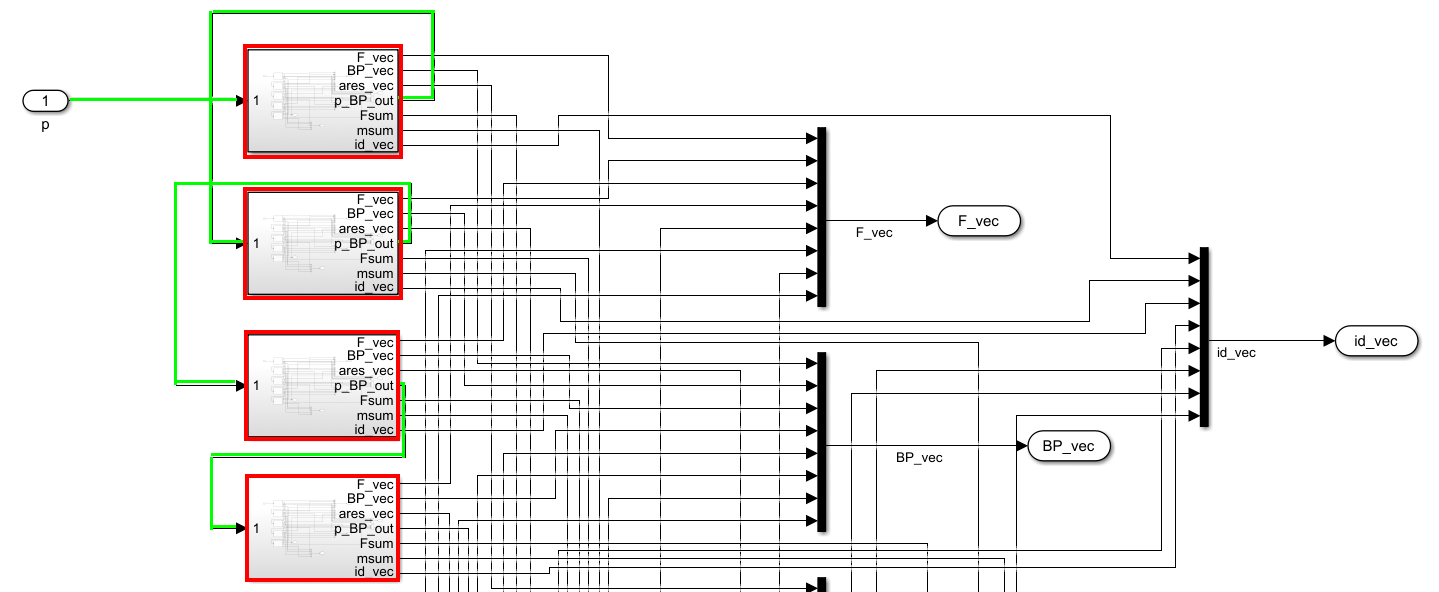
\includegraphics[width=\linewidth]{./pic/expandedmodel_brakepipe}
	\caption{Expanded Model - Brake Pipe}
	\label{fig:expandedmodel_brakepipe}
\end{figure}

\par\noindent
Figure \ref{fig:expandedmodel_brakepipe} shows how the wagons (marked by red rectangles) are interconnected by the brake pipe (marked by green arrows). This is analogous to how the wagons were connected in the initial model from section \ref{sec:InitialModel}.  

\begin{figure}[H]
	\centering
	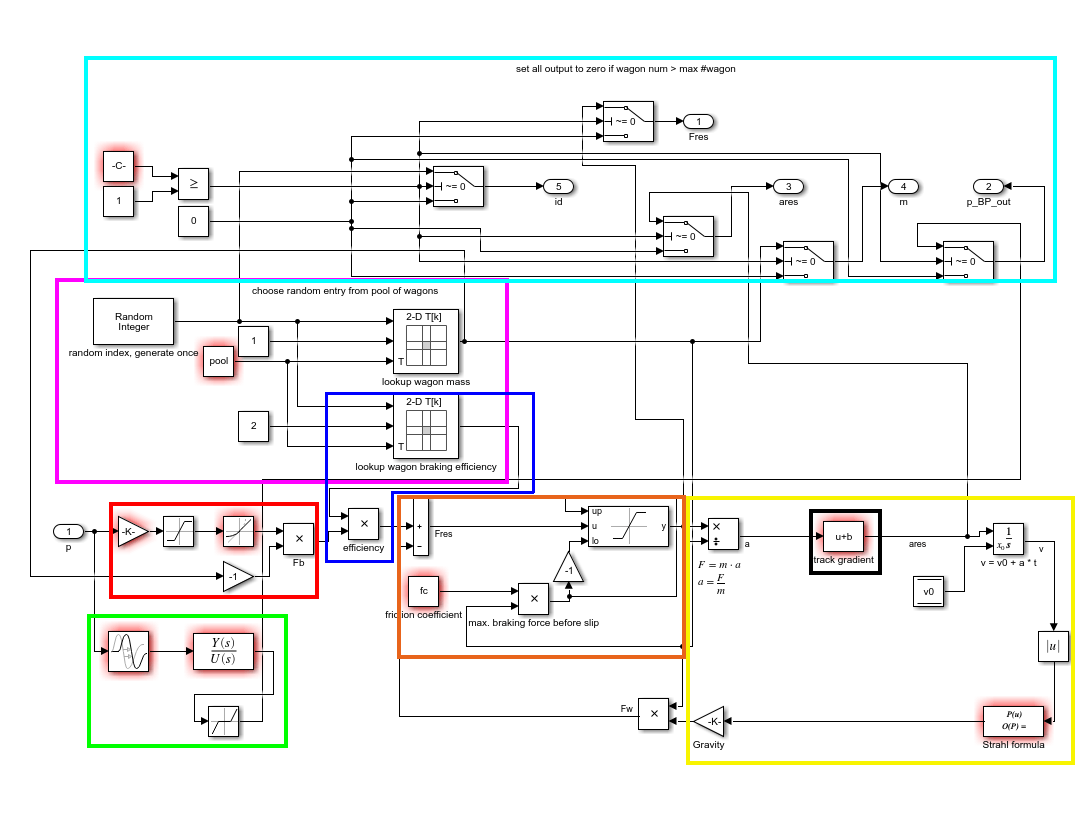
\includegraphics[width=\linewidth]{./pic/expandedmodel_wagon}
	\caption{Expanded Model - Wagon}
	\label{fig:expandedmodel_wagon}
\end{figure}

\par\noindent
Figure \ref{fig:expandedmodel_wagon} shows the expanded model of the freight wagon. There are components which have remained largely unchanged, while others have been added or altered to account for for the changes required to implement ${\mathcal{M}}$. To recapitulate, the initial model's freight wagon comprised of three components: The brake cylinder ${\mathcal{M}}_{bc}$, the brake pipe ${\mathcal{M}}_{bp}$, and the driving resistance. The implementation of the brake pipe has remained largely unchanged, the only exception being the addition of a dead zone to filter out very small values of $p_{bp}$, ranging from $-0.005$ to $0.005$. This was necessary as these small values interfered with the simulation result in a negative way. The implementation of the brake pipe ${\mathcal{M}}_{bp}$ is marked by the green rectangle.
\par
The implementation of the brake cylinder ${\mathcal{M}}_{bc}$ has also remained largely unchanged from the initial model, though the wagon's mass used to calculate $F_{b,max}$ is now read dynamically rather than being a static value (more on this later). The brake cylinder is marked by the red rectangle. The implementation of the calculation of the train's driving resistance has too remained unchanged except for the wagon's mass, used to determine the acceleration, being read dynamically, analogous to the brake cylinder. This component is marked by the yellow rectangle.
\bigskip
\par\noindent
According to the definition of ${\mathcal{M}}$, the following factors still need to be accounted for: The wagon mass $m$, the train composition $comp$, the track gradient $\alpha$, and the wheel/rail friction coefficient $\mu$. It is therefore necessary to add new components implementing these to the wagon model.
\par
While the initial model's wagons did indeed have a mass, it had a static value, and it was the same for all 40 wagons, making them identical and indistinguishable from one another. This is of course undesirable as it poorly reflects reality. To make up for this flaw, a pool of 500 wagons has been randomly generated via a python script:

\bigskip
\begin{python}
import csv
import random

with open('pool.csv', 'w', newline='') as pool:
	fieldnames = ['Wagon_ID', 'Mass', 'Braking_eff']
	writer = csv.DictWriter(pool, fieldnames=fieldnames)
	
	writer.writeheader()
	for i in range(0,500): 
		mass = random.randrange(12000, 90000, 100)
		braking_eff = round(random.uniform(0.75, 0.95),2)
		writer.writerow({'Wagon_ID': i, 'Mass': mass, 'Braking_eff': braking_eff})
\end{python}
\bigskip

\noindent
This creates a table with 500 entries of the following structure:

\bigskip
\begin{table}[H]
	\label{tab:wagonpool}
	\centering
	\begin{tabular}{c|c|c}
		Wagon\_ID & Wagon Mass & Braking Efficiency \\
		\hline
		0 & 53800 & 0.83 \\
		\hline
		1 & 60800 & 0.77 \\
		\hline
		... & ... & ... \\
		\hline
		499 & 66600 & 0.81 \\
	\end{tabular}
	\caption{Wagon pool structure}
\end{table}

\bigskip

\noindent
Each wagon contained in the pool is identifiable by its ID and has the properties wagon mass and braking efficiency, i.e. a characteristic for the integrity of its brakes. Both properties are randomly generated for each wagon, the mass being assigned a value between 12000 and 90000 kilograms (with a step size of 100 kilograms), and the braking efficiency following a uniform distribution between 75 and 95 percent integrity. In order to read the values from the table, during simulation, each of the 40 wagon subsystems generates a random index between 0 and 499, i.e. each wagon is assigned an ID. By utilizing two direct lookup table blocks, the row with the assigned ID is selected, and the corresponding values for mass and braking efficiency are read from the table. The implementation of this component is marked by the pink rectangle. The value of $m$ is then used to calculate $F_{b}$, $a$, the driving resistance, the maximum braking force before slip, and the overall mass of the train $m_{total}$. The value of the braking efficiency is multiplied with $F_{b}$, meaning a lower integrity will result in a lower effective braking force. This component is marked by the blue polygon.
\par
The next element of ${\mathcal{V}}$ to address is the train composition $comp$. In the initial model, $comp$ is static, meaning the train is always comprised of 40 identical wagons. There is now a system in place that allows for wagons with diverse properties; we now need to design a system that allows for a variable number of wagons. In the simulink model, the train is made up of 40 subsystems, each representing one freight wagon. The obvious approach would be only having as many of these systems as desired, e.g. for a train consisting of 27 wagons, there would only be 27 wagon subsystems in the model. Since simulink however offers no straightforward way of adding or removing subsystems during simulation, a workaround is necessary. The solution taken here is using switch blocks to set output to zero for all unwanted subsystems, effectively removing their impact on the simulation. Each of the 40 models is assigned a constant representing their position; for each simulation, the desired number of wagons the train should encompass is specified as simulation input. During simulation, each subsystem compares this value to its position index. If their index is greater than the desired number of wagons, the switch blocks are set to output zero. For example, take a train of 15 wagons. The subsystems with position indices one to 15 will produce output, and the subsystems with indices 16 to 40 will not. This component is marked by the cyan rectangle.
\par
The track gradient $\alpha$ is used to calculate the additional braking or traction force resulting from the track's pitch angle. 

\begin{equation}
\label{eq:inclinationforce}
F_{N} = G_{F,Z} \cdot f_{N}
\end{equation}

\noindent
Equation \ref{eq:inclinationforce} is used to calculate the inclination force $F_{N}$, where $G_{F,Z} = m \cdot 9.81$ is the weight force acting on the wagon, and $f_{N} = \sin(\alpha)$ is the inclination force number [wende, 95]. Accordingly, this force is calculated during simulation and then added to (or subtracted from) the generated braking force $F_{b}$ to determine the effective braking force, taking into account the slope of the train track. This component is marked by the black rectangle.
\par
As mentioned in chapter \ref{chap:FundamentalsOfRailwayVehicleEngineering}, the wheel/rail friction coefficient $\mu$ determines how much braking force may be applied before sliding occurs, negatively impacting the braking performance. Since the exact mechanics of how sliding affects the braking process go beyond the scope of this work, a different approach has been chosen to incorporate $\mu$.

\begin{equation}
\label{eq:frictioncoefficient}
F_{b,e} = F_{b,max} \cdot \mu
\end{equation}

\noindent
Equation \ref{eq:frictioncoefficient} is used to calculate the braking force before sliding would occur, $F_{b,e}$ by multiplying the maximum possible braking force $F_{b,max}$ with the wheel/rail friction coefficient $\mu$. The result is then used to limit the applied braking force $F_{b}$ so that sliding is avoided, utilizing a saturation dynamic block. This still satisfies $R_{\mu,F_{b}} \in \{ {\mathcal{R}} \}$. This component is marked by the brown rectangle.
\bigskip
\par\noindent
This completes the description of the simulink model. Reaching back to chapter \ref{chap:FundamentalsOfRailwayVehicleEngineering}, all elements of $\{ {\mathcal{V}} \}$, $\{ {\mathcal{R}} \}$ and $\{ c \}$ have been accounted for, and we can therefore conclude our theoretical model ${\mathcal{M}}$ has been implemented. It may now be used for simulation and data generation.

\section{Outlook}
\label{sec:Outlook}

\par\noindent
While the model defined in chapter \ref{chap:FundamentalsOfRailwayVehicleEngineering} satisfies the requirements for this work, there are many more factors that might be incorporated in order to achieve a more accurate representation of reality. Some of these factors shall be discussed here briefly. So far, the generated braking force $F_{b}$ is calculated by transforming the braking pressure $p_{bp}$ into a coefficient, and applying that coefficient to the maximum braking capacity $F_{b,max}$.

\begin{equation}
\label{eq:brakingforceadjusted}
F_{b} = \xi \cdot \sum P_{N}
\end{equation}

\noindent
Equation \ref{eq:brakingforceadjusted} offers a more detailed way of calculating $F_{b}$, where $\sum P_{N}$ is the sum of all applying forces actuating the brake shoes on the wheel tread, or the brake pads against the discs, respectively; the proportionality coefficient $\xi$ might be the friction coefficient between the brake shoes and the wheel, or

\begin{equation}
\label{eq:xi}
\xi = \frac{4 \cdot r_{m}}{D_{o}} \cdot \mu_{d}
\end{equation}

\noindent
for disc brakes, where $r_{m}$ is the medium friction radius, $D_{o}$ is the wheel diameter, and $\mu_{d}$ is the friction coefficient between brake pad and disk [train braking, 23].
\par
As the focus of this work lies on the braking process, the modeling of traction force is kept rather simple. It might however be desirable to create a more sophisticated model, in order to achieve a more realistic result. For example, as of right now, the applied traction force depends only on the discrepancy between current and maximum velocity; in reality, the maximum traction force is also limited by wheel/rail adhesion just as the braking force is [wende, 157]. One might also want to factor in differences between various engines.